\documentclass{beamer}

\usepackage{amsmath}
\usepackage{amssymb}
\usepackage{amsthm}
\usepackage{bpextra}
\usepackage{float}
\usepackage{geometry}
\usepackage{latexsym}
\usepackage{natbib}
\usepackage{pdfpages}
\usepackage{subcaption}
\usepackage{tikz}
\usepackage{tkz-berge}
\usepackage{varwidth}

% tikz things
\usetikzlibrary{petri, topaths, positioning, decorations.pathmorphing}

% natbib source
\bibliographystyle{agsm}
\renewcommand{\bibsection}{}

\pgfarrowsdeclare{arr}{arr}{
    \setlength{\arrowsize}{2\pgflinewidth}
    \addtolength{\arrowsize}{.5\pgflinewidth}
    \pgfarrowsrightextend{-1\arrowsize}
    \pgfarrowsleftextend{1\arrowsize}
}{
    \setlength{\arrowsize}{2\pgflinewidth}
    \addtolength{\arrowsize}{.5\pgflinewidth}
    \pgfpathmoveto{\pgfpoint{-5\arrowsize}{4\arrowsize}}
    \pgfpathlineto{\pgfpointorigin}
    \pgfpathlineto{\pgfpoint{-5\arrowsize}{-4\arrowsize}}
    \pgfusepathqstroke
}

\newcommand{\drawsquig}{\draw[-arr,
line join=round,
decorate, decoration={
    zigzag,
    segment length=4,
    amplitude=.9,post=lineto,
    post length=2pt
}]}

\newenvironment{scprooftree}[1]%
  {\gdef\scalefactor{#1}\begin{center}\proofSkipAmount \leavevmode}%
  {\scalebox{\scalefactor}{\DisplayProof}\proofSkipAmount \end{center} }


\newcommand\vc[1]{\vcenter{\hbox{#1}}}

\newcommand\atom[1]{%
 \ifx#11a\else%
 \ifx#12b\else%
 \ifx#13c\else%
 \fi\fi\fi
}

\newcommand\0{0}
\newcommand\1{1}
\newcommand\+{+}
\renewcommand\*{\times}

\newcommand{\tightplus}{\!+\!}
\newcommand{\tighttimes}{\!\*\!}
\newcommand\subs[1]{\mathsf{|#1|}}

\tikzstyle{tok}=[circle,inner sep=0pt,minimum size=4pt,outer sep=1pt]
\tikzstyle{src}=[black,text height=1ex,text depth=0ex,rotate=90]
\tikzstyle{tgt}=[black,text height=1ex,text depth=0ex]%,rotate=-45]
\tikzstyle{for}=[text height=1.5ex,text depth=.25ex]
\tikzstyle{jmp}=[->,line width=1pt,cap=round,gray]
\tikzstyle{jmp1}=[jmp]
\tikzstyle{jmp2}=[jmp,red]

\tikzstyle{tokB}=[fill,tok]
\tikzstyle{tokG}=[fill,tok,gray]
\tikzstyle{tokR}=[fill,tok,red]
\tikzstyle{tokRed}=[fill,tok,red]
\tikzstyle{tokBlue}=[fill,tok,blue]
\tikzstyle{tokGreen}=[fill,tok,darkgreen]
\tikzstyle{tokF}=[draw,thick,gray,circle,inner sep=0pt, minimum size=7pt]

\tikzstyle{matrix}=[x=-5mm,y=5mm,rotate=-90]

% delta-equals (unused)
\def\deltaeq{\mathrel{\ensurestackMath{\stackon[1pt]{=}{\scriptstyle\Delta}}}}
% define-equals
\def\defeq{::=}
% set-to-equals
\def\seteq{:=}

\newcommand\dual{\overline}

\title{From Additive to Classical Proof Search}
\date{}


\author{Adam Lassiter \and Willem Heijltjes\\Department of Computer Science\\University of Bath}

\begin{document}

    \frame{
        \titlepage
    }


    \frame{
        \frametitle{Introduction}
        
        Outline:
        \begin{itemize}
            \item Additive Linear Logic (ALL)
            \item Proof search in ALL through \emph{coalescence}
            \item Classical Logic (CL)
            \item Proof search in CL through \emph{coalescence} and \emph{additive stratification}
            \item Complexity bounds of proof search
            \item Dimensionality of CL formulae
        \end{itemize}
    }



    \frame{
        \frametitle{Additive Linear Logic (ALL)}

        \[ A, B, C \quad \defeq \quad 0 \mid 1 \mid a \mid \dual a \mid A + B \mid A \* B \]
        
        \begin{itemize}
            \item $0, a, \+$ are duals of $1, \dual a, \*$ respectively
        \end{itemize}
    }

    \frame{
        \frametitle{Additive Linear Logic (ALL)}
        
        Some examples:
        \begin{itemize}
            \item $(\atom1 \+ \dual{\atom2}) \* 1$ is the dual of $(\dual{\atom1} \* \atom2) \+ 0$ and vice versa
            \item %TODO More examples
        \end{itemize}
    }

    \frame{
        \frametitle{Additive Linear Logic (ALL)}

        \begin{figure}
            \centering
            \begin{minipage}{0.3\linewidth}
                \begin{prooftree}
                    \AxiomC{~}
                    \RightLabel{$ax$}
                    \UnaryInfC{$\vdash a,\dual a$}
                \end{prooftree}
            \end{minipage}
            \begin{minipage}{0.3\linewidth}
                \begin{prooftree}
                    \AxiomC{~}
                    \RightLabel{$\1$}
                    \UnaryInfC{$\vdash \1,A$}
                \end{prooftree}
            \end{minipage}
            \begin{minipage}{0.3\linewidth}
                \begin{prooftree}
                    \AxiomC{$\vdash A,C$}
                    \RightLabel{$\+_1$}
                    \UnaryInfC{$\vdash A\+B,C$}
                \end{prooftree}
            \end{minipage}
        \end{figure}

        \begin{figure}
            \begin{minipage}{0.4\linewidth}
                \begin{prooftree}
                    \AxiomC{$\vdash B,C$}
                    \RightLabel{$\+_2$}
                    \UnaryInfC{$\vdash A\+B,C$}
                \end{prooftree}
            \end{minipage}
            \begin{minipage}{0.4\linewidth}
                \begin{prooftree}
                    \AxiomC{$\vdash A,C$}
                    \AxiomC{$\vdash B,C$}
                    \RightLabel{$\*$}
                    \BinaryInfC{$\vdash A\*B,C$}
                \end{prooftree}
            \end{minipage}
        \end{figure}

        \begin{itemize}
            \item All sequents are comprised of a pair of terms, maintained by deduction rules
        \end{itemize}
    }

    \frame{
        \frametitle{Additive Linear Logic (ALL)}

        Example: $\vdash \atom1 \* \atom2, \dual{\atom1} \+ \dual{\atom2}$
        \begin{prooftree}
            \AxiomC{$~$}
            \RightLabel{$ax$}\UnaryInfC{$\vdash \atom1, \dual{\atom1}$}
            \RightLabel{$\+$}\UnaryInfC{$\vdash \atom1, \dual{\atom1} \+ \dual{\atom2}$}
            \AxiomC{$~$}
            \RightLabel{$ax$}\UnaryInfC{$\vdash \atom2, \dual{\atom2}$}
            \RightLabel{$\+$}\UnaryInfC{$\vdash \atom2, \dual{\atom1} \+ \dual{\atom2}$}
            \RightLabel{$\*$}\BinaryInfC{$\vdash \atom1 \* \atom2, \dual{\atom1} \+ \dual{\atom2}$}
        \end{prooftree}
    }



    \frame{
        \frametitle{Coalescence}
        
        Spawning:
        \[
            \vc{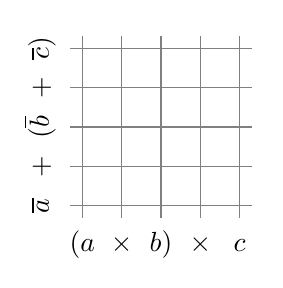
\begin{tikzpicture}[matrix]
                \foreach \x/\a in {1/\dual{\atom1}, 2/\+, 3/(\dual{\atom2}, 4/\+, 5/\dual{\atom3})}%
                    \draw[gray] (\x,0) node[src] {$\a$} (\x,.7) -- (\x,5.3);
                \foreach \y/\b in {1/(\atom1, 2/\*, 3/\atom2), 4/\*, 5/\atom3}%
                    \draw[gray] (0,\y) node[tgt] {$\b$} (.7,\y) -- (5.3,\y);
            \end{tikzpicture}}
            \quad\rightsquigarrow\quad
            \vc{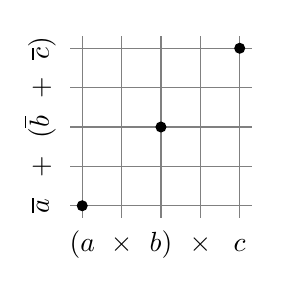
\begin{tikzpicture}[matrix]
                \foreach \x/\a in {1/\dual{\atom1}, 2/\+, 3/(\dual{\atom2}, 4/\+, 5/\dual{\atom3})}%
                    \draw[gray] (\x,0) node[src] {$\a$} (\x,.7) -- (\x,5.3);
                \foreach \y/\b in {1/(\atom1, 2/\*, 3/\atom2), 4/\*, 5/\atom3}%
                    \draw[gray] (0,\y) node[tgt] {$\b$} (.7,\y) -- (5.3,\y);
                \foreach \p/\n in { {1,1}/a1, {3,3}/b1, {5,5}/c1} \node[tokB] (\n) at (\p) {};
            \end{tikzpicture}}
        \]

        \begin{itemize}
            \item Corresponds to axiom rule for ALL
        \end{itemize}

    }

    \frame{
        \frametitle{Coalescence}

        Transitions:
        \[
            \def\dual{}
            \begin{array}{ccc}
                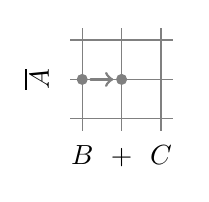
\begin{tikzpicture}[matrix]
                    \foreach \i/\a in {1/{}, 2/\dual A, 3/{}}
                        {\draw[gray] (\i,0) node[src] {$\a$} (\i,.7) -- (\i,3.3);}
                    \foreach \j/\b in {1/B, 2/\+, 3/C}
                        {\draw[gray] (0,\j) node[tgt] {$\b$} (.7,\j) -- (3.3,\j);}
                    \node[tokG] (a) at (2,1) {};
                    \node[tokG] (c) at (2,2) {};
                    \draw[jmp1] (a) to (c);
                \end{tikzpicture}
                &
                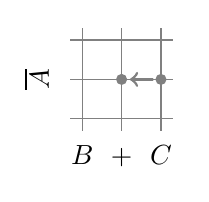
\begin{tikzpicture}[matrix]
                    \foreach \i/\a in {1/{}, 2/\dual A, 3/{}}
                        {\draw[gray] (\i,0) node[src] {$\a$} (\i,.7) -- (\i,3.3);}
                    \foreach \j/\b in {1/B, 2/\+, 3/C}
                        {\draw[gray] (0,\j) node[tgt] {$\b$} (.7,\j) -- (3.3,\j);}
                    \node[tokG] (b) at (2,3) {};
                    \node[tokG] (c) at (2,2) {};
                    \draw[jmp1] (b) to (c);
                \end{tikzpicture}
                &
                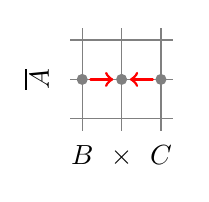
\begin{tikzpicture}[matrix]
                  \foreach \i/\a in {1/{}, 2/\dual A, 3/{}}
                    {\draw[gray] (\i,0) node[src] {$\a$} (\i,.7) -- (\i,3.3);}
                  \foreach \j/\b in {1/B, 2/\*, 3/C}
                    {\draw[gray] (0,\j) node[tgt] {$\b$} (.7,\j) -- (3.3,\j);}
                  \node[tokG] (a) at (2,1) {};
                  \node[tokG] (b) at (2,3) {};
                  \node[tokG] (c) at (2,2) {};
                  \draw[jmp2] (a) to (c);
                  \draw[jmp2] (b) to (c);
                \end{tikzpicture}
                \\
                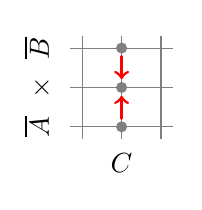
\begin{tikzpicture}[matrix]
                    \foreach \i/\a in {1/\dual A, 2/\*, 3/\dual B}
                        {\draw[gray] (\i,0) node[src] {$\a$} (\i,.7) -- (\i,3.3);}
                    \foreach \j/\b in {1/{}, 2/C, 3/{}}
                        {\draw[gray] (0,\j) node[tgt] {$\b$} (.7,\j) -- (3.3,\j);}
                    \node[tokG] (a) at (1,2) {};
                    \node[tokG] (b) at (3,2) {};
                    \node[tokG] (c) at (2,2) {};
                    \draw[jmp2] (a) to (c);
                    \draw[jmp2] (b) to (c);
                \end{tikzpicture}
                &
                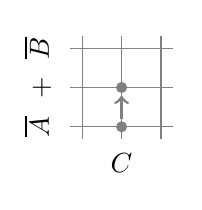
\begin{tikzpicture}[matrix]
                    \foreach \i/\a in {1/\dual A, 2/\+, 3/\dual B}
                        {\draw[gray] (\i,0) node[src] {$\a$} (\i,.7) -- (\i,3.3);}
                    \foreach \j/\b in {1/{}, 2/C, 3/{}}
                        {\draw[gray] (0,\j) node[tgt] {$\b$} (.7,\j) -- (3.3,\j);}
                    \node[tokG] (a) at (1,2) {};
                    \node[tokG] (c) at (2,2) {};
                    \draw[jmp1] (a) to (c);
                \end{tikzpicture}
                &
                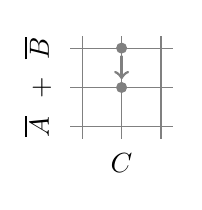
\begin{tikzpicture}[matrix]
                    \foreach \i/\a in {1/\dual A, 2/\+, 3/\dual B}
                        {\draw[gray] (\i,0) node[src] {$\a$} (\i,.7) -- (\i,3.3);}
                    \foreach \j/\b in {1/{}, 2/C, 3/{}}
                        {\draw[gray] (0,\j) node[tgt] {$\b$} (.7,\j) -- (3.3,\j);}
                    \node[tokG] (b) at (3,2) {};
                    \node[tokG] (c) at (2,2) {};
                    \draw[jmp1] (b) to (c);
                \end{tikzpicture}
            \end{array}
        \]
        
        \begin{itemize}
            \item Corresponds to sequent rules for ALL
        \end{itemize}
    }

    \frame{
        \frametitle{Coalescence}

        Example:
        \[
            \vc{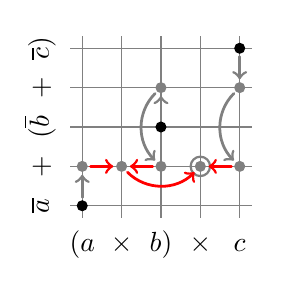
\begin{tikzpicture}[matrix]
                \foreach \x/\a in {1/\dual{\atom1}, 2/\+, 3/(\dual{\atom2}, 4/\+, 5/\dual{\atom3})}%
                    \draw[gray] (\x,0) node[src] {$\a$} (\x,.7) -- (\x,5.3);
                \foreach \y/\b in {1/(\atom1, 2/\*, 3/\atom2), 4/\*, 5/\atom3}%
                    \draw[gray] (0,\y) node[tgt] {$\b$} (.7,\y) -- (5.3,\y);
                \foreach \p/\n in {
                    {2,1}/a2, {2,2}/ab,
                    {4,3}/b2, {2,3}/b3,
                    {4,5}/c2, {2,5}/c3%
                } \node[tokG] (\n) at (\p) {};
                \node[tokG] (abc) at (2,4) {};
                \node[circle,draw,gray,thick,inner sep=0pt,minimum size=7pt] at (2,4) {};
                \foreach \p/\n in { {1,1}/a1, {3,3}/b1, {5,5}/c1} \node[tokB] (\n) at (\p) {};
                \foreach \s/\t in { a1/a2, b1/b2, c1/c2} \draw[jmp1] (\s)--(\t);
                \foreach \s/\t in { a2/ab, b3/ab, c3/abc} \draw[jmp2] (\s)--(\t);
                \draw[jmp1,bend right=45] (b2) to (b3);
                \draw[jmp1,bend right=45] (c2) to (c3);
                \draw[jmp2,bend right=45] (ab) to (abc);
            \end{tikzpicture}}
        \]

        \begin{itemize}
            \item Algorithm succeeds if and only if there is an ALL proof of the given formula, see \citet{petri-nets}
        \end{itemize}
    }



    \frame{
        \frametitle{Classical Logic (CL)}

        \[
            A, B, C \quad \defeq \quad \top \mid \bot \mid a \mid \dual a \mid A \vee B \mid A \wedge B
        \]
    }

    \frame{
        \frametitle{Classical Logic (CL)}

        \begin{figure}[H]
            \centering
            \begin{minipage}[H]{.3\linewidth}
                \begin{prooftree}
                    \AxiomC{~}
                    \RightLabel{$\top$}
                    \UnaryInfC{$\vdash \top$}
                \end{prooftree}
            \end{minipage}
            \begin{minipage}[H]{.3\linewidth}
                \begin{prooftree}
                    \AxiomC{$\vdash \Gamma, A$}
                    \RightLabel{$\vee$}
                    \UnaryInfC{$\vdash \Gamma, A \vee B$}
                \end{prooftree}
            \end{minipage}
            \begin{minipage}[H]{.3\linewidth}
                \begin{prooftree}
                    \AxiomC{$\vdash \Gamma$}
                    \RightLabel{$w$}
                    \UnaryInfC{$\vdash \Gamma, A$}
                \end{prooftree}
            \end{minipage}

            \begin{minipage}[H]{.3\linewidth}
                \begin{prooftree}
                    \AxiomC{~}
                    \RightLabel{$ax$}
                    \UnaryInfC{$\vdash a, \dual a$}
                \end{prooftree}
            \end{minipage}
            \begin{minipage}[H]{.3\linewidth}
                \begin{prooftree}
                    \AxiomC{$\vdash \Gamma, A$}
                    \AxiomC{$\vdash \Gamma, B$}
                    \RightLabel{$\wedge$}
                    \BinaryInfC{$\vdash \Gamma, A \wedge B$}
                \end{prooftree}
            \end{minipage}
            \begin{minipage}[H]{.3\linewidth}
                \begin{prooftree}
                    \AxiomC{$\vdash \Gamma, A, A$}
                    \RightLabel{$c$}
                    \UnaryInfC{$\vdash \Gamma, A$}
                \end{prooftree}
            \end{minipage}
        \end{figure}

        \begin{itemize}
            \item $A, B, C$ are formulae, $\Gamma, \Delta, \Sigma$ are sequents
            \item $\wedge, \vee$ rules preserve the number of terms in a sequent
        \end{itemize}
    }

    \frame{
        \frametitle{Classical Logic (CL)}

        Example: % TODO: CL sequent proof example
    }



    \frame{
        \frametitle{Additive Stratification}

        \begin{prooftree}
            \AxiomC{}
            \RightLabel{$\top, ax$}\doubleLine\UnaryInfC{$\vdash A_1$}
            \RightLabel{$w$}\doubleLine\UnaryInfC{$\vdash \Gamma_1$}
            \AxiomC{\dots}
            \AxiomC{}
            \RightLabel{$\top, ax$}\doubleLine\UnaryInfC{$\vdash A_n$}
            \RightLabel{$w$}\doubleLine\UnaryInfC{$\vdash \Gamma_n$}
            \RightLabel{$\wedge, \vee$}\doubleLine\TrinaryInfC{$\vdash P \dots P$}
            \RightLabel{$c$}\doubleLine\UnaryInfC{$\vdash P$}
        \end{prooftree}
        \begin{itemize}
            \item Rearrangement does not affect the number of terms in sequents
            \item Does not work for MLL rules, see \citet{contraction-restrictions}
        \end{itemize}
    }

    \frame{
        \frametitle{Additive Stratification}

        \begin{figure}[H]
            \centering
            \begin{minipage}[H]{0.4\linewidth}
                \begin{prooftree}
                    \AxiomC{$\vdash \Gamma, A$}
                    \RightLabel{$\vee$}\UnaryInfC{$\vdash \Gamma, A \vee B$}
                    \RightLabel{$w$}\UnaryInfC{$\vdash \Gamma, A \vee B$, C}
                \end{prooftree}
            \end{minipage}
            $\leadsto$
            \begin{minipage}[H]{0.4\linewidth}
                \begin{prooftree}
                    \AxiomC{$\vdash \Gamma, A$}
                    \RightLabel{$w$}\UnaryInfC{$\vdash \Gamma, A, C$}
                    \RightLabel{$\vee$}\UnaryInfC{$\vdash \Gamma, A \vee B, C$}
                \end{prooftree}
            \end{minipage}
        \end{figure}
        
        \begin{figure}[H]
            \centering
            \begin{minipage}[H]{0.4\linewidth}
                \begin{prooftree}
                    \AxiomC{$\vdash \Gamma, A$}
                    \AxiomC{$\vdash \Gamma, B$}
                    \RightLabel{$\wedge$}\BinaryInfC{$\vdash \Gamma, A \wedge B$}
                    \RightLabel{$w$}\UnaryInfC{$\vdash \Gamma, A \wedge B, C$}
                \end{prooftree}
            \end{minipage}
            $\leadsto\quad$
            \begin{minipage}[H]{0.4\linewidth}
                \begin{prooftree}
                    \AxiomC{$\vdash \Gamma, A$}
                    \RightLabel{$w$}\UnaryInfC{$\vdash \Gamma, A, C$}
                    \AxiomC{$\vdash \Gamma, B$}
                    \RightLabel{$w$}\UnaryInfC{$\vdash \Gamma, B, C$}
                    \RightLabel{$\wedge$}\BinaryInfC{$\vdash \Gamma, A \wedge B, C$}
                \end{prooftree}
            \end{minipage}
        \end{figure}

        \begin{figure}[H]
            \centering
            \begin{minipage}[H]{0.4\linewidth}
                \begin{prooftree}
                    \AxiomC{$\vdash \Gamma, A, A$}
                    \RightLabel{$c$}\UnaryInfC{$\vdash \Gamma, A$}
                    \RightLabel{$w$}\UnaryInfC{$\vdash \Gamma, A, B$}
                \end{prooftree}
            \end{minipage}
            $\leadsto\quad$
            \begin{minipage}[H]{0.4\linewidth}
                \begin{prooftree}
                    \AxiomC{$\vdash \Gamma, A, A$}
                    \RightLabel{$w$}\UnaryInfC{$\vdash \Gamma, A, A, B$}
                    \RightLabel{$c$}\UnaryInfC{$\vdash \Gamma, A, B$}
                \end{prooftree}
            \end{minipage}
        \end{figure}
    }

    \frame{
        \frametitle{Additive Stratification}

        \begin{figure}[H]
            \centering
            \begin{minipage}[H]{0.4\linewidth}
                \begin{prooftree}
                    \AxiomC{$\vdash \Gamma, A, A$}
                    \RightLabel{$c$}\UnaryInfC{$\vdash \Gamma, A$}
                    \RightLabel{$\vee$}\UnaryInfC{$\vdash \Gamma, A \vee B$}
                \end{prooftree}
            \end{minipage}
            $\leadsto$
            \begin{minipage}[H]{0.4\linewidth}
                \begin{prooftree}
                    \AxiomC{$\vdash \Gamma, A, A$}
                    \RightLabel{$\vee$}\UnaryInfC{$\vdash \Gamma, A \vee B, A$}
                    \RightLabel{$\vee$}\UnaryInfC{$\vdash \Gamma, A \vee B, A \vee B$}
                    \RightLabel{$c$}\UnaryInfC{$\vdash \Gamma, A \vee B$}
                \end{prooftree}
            \end{minipage}
        \end{figure}

        \begin{figure}[H]
            \centering
            \begin{minipage}[H]{0.3\linewidth}
                \begin{scprooftree}{0.8}
                    \AxiomC{$\vdash \Gamma, A, A$}
                    \RightLabel{$c$}\UnaryInfC{$\vdash \Gamma, A$}
                    \AxiomC{$\vdash \Gamma, B$}
                    \RightLabel{$\wedge$}\BinaryInfC{$\vdash \Gamma, A \wedge B$}
                \end{scprooftree}
            \end{minipage}
            $\leadsto\quad$
            \begin{minipage}[H]{0.6\linewidth}
                \begin{scprooftree}{0.8}
                    \AxiomC{$\vdash \Gamma, A, A$}
                    \AxiomC{$\vdash \Gamma, B$}
                    \RightLabel{$w$}\UnaryInfC{$\vdash \Gamma, A, B$}
                    \RightLabel{$\wedge$}\BinaryInfC{$\vdash \Gamma, A, A \wedge B$}
                    \AxiomC{$\vdash \Gamma, B$}
                    \RightLabel{$w$}\UnaryInfC{$\vdash \Gamma, B, A \wedge B$}
                    \RightLabel{$\wedge$}\BinaryInfC{$\vdash \Gamma, A \wedge B, A \wedge B$}
                    \RightLabel{$c$}\UnaryInfC{$\vdash \Gamma, A \wedge B$}
                \end{scprooftree}
            \end{minipage}
        \end{figure}

        \begin{itemize}
            \item Proof trees are described as \emph{morally equivalent}, see \citet{proofs-and-types}
        \end{itemize}
    }

    \frame{
        \frametitle{Additive Stratification}

        Example:
        %TODO: Additive stratification example
    }



    \frame{
        \frametitle{Coalescence in CL}

        We investigate how the coalescence technique applies to classical propositional logic.
        The main idea is that a classical formula $A$ can be proved by additive rules applied to a sequent $\vdash A,\dots,A$ with $n$ copies of $A$.
        This is easily shown by a \emph{stratification} of sequent proofs with additive rules, where all contractions are pushed to the bottom (conclusion), and weakenings to the top (axioms).

        Correspondingly, we generalize coalescence proof search to CL by applying it to a grid of $n$ dimensions, for any $n$, where it was previously fixed at $2$.
        The algorithm will start at dimension $1$, and when it fails at dimension $n$ it will try again at dimension $n+1$, up to a theoretically determined upper bound.
        
        % TODO: Example in 1D, 2D, lines & squares for 3D?
    }    
       
    \frame{
        \frametitle{Coalescence in CL}

        For a formula $P$ in CL, the coalescence algorithm runs as follows:
        \begin{enumerate}
            \item Set $n := 1$
            \item\label{l} Construct the $n$-dimensional grid of possible $n$-term sequents $\vdash A_1 \dots A_n \in \subs A \* \dots_n \* \subs A$
            \item Spawn tokens at all instances of axiom links $\vdash \Gamma, a, \dual a$
            \item Exhaustively perform transitions given by the CL sequent calculus rules
            \item Does there exist a token at $(P, P \dots P) \equiv \,\, \vdash P, P \dots P \equiv \,\, \vdash P$?
            \begin{enumerate}
                \item Yes --- Halt with a proof for $P$ and dimensionality $n$
                \item No --- Increment $n := n + 1$ and goto~\ref{l}
            \end{enumerate}
        \end{enumerate}
    }



    \frame{
        \frametitle{Questions}
        
        % TODO: upper bound on dimension, what is a good representation for (matrix | tokens | ...)
    }



    \frame{
        \frametitle{Dimensionality}

        The dimensionality of a proof is then the dimensionality of our grid when the root is reached, equivalent to the number of contractions required in an equivalent sequent proof.
        A CL formula can thus be proved by an $n$-dimensional additively stratified proof, where $n$ is the number of terms in a sequent before contraction.
        Through a natural transformation on steps of the algorithm to equivalent sequent proofs, coalescence up to $n = N$ is then exactly (additively stratified) proof search, with implicit weakening and contraction of all sequents up to $N$ terms.
    }



    \frame{
        \frametitle{Conclusion}
    }



    \frame{
        \frametitle{References}
        \bibliography{dortmund}
    }

\end{document}
